\chapter{\IfLanguageName{dutch}{Stand van zaken}{State of the art}}
\label{ch:stand-van-zaken}

% Tip: Begin elk hoofdstuk met een paragraaf inleiding die beschrijft hoe
% dit hoofdstuk past binnen het geheel van de bachelorproef. Geef in het
% bijzonder aan wat de link is met het vorige en volgende hoofdstuk.

% Pas na deze inleidende paragraaf komt de eerste sectiehoofding.

\section{What is a Front-end framework?}

A front-end framework is a paradigm of best practices and provides a certain approach to develop the front-end of an application.
Lots of webapplications share the same base features. A framework bundles these features and provides tool to easily develop them in a structured way. Web frameworks help us achieve structure in our applications and give developers a place to start and therefore leads to accelerated development. By defining several rules and best practices, a codebase is easier to understand for other developers when they have knowledge of the framework. \autocite{Spittel}

\section{Multiple-page vs single-page applications}

The classic approach of multiple-page applications (MPA) has the following flow:
\begin{enumerate}
    \item A user performs an action
    \item The client sends a request to the server
    \item The server consumes the action
    \item The server sends a new page to the client
    \item The client reloads the page
\end{enumerate}
With this approach the client always gets new pages and causes a reload on every user action.
When using a sngle-page application (SPA), the client downloads the application at first and the rendering happens on the client side. This way the page does not need a refresh on every user action. Though the client still communicates with the server for data, not for handling pages.
Given this we can state that an MPA uses server side rendering, while an SPA renders on the client side.
\autocite{Skolski}

\section{What is Angular?}
\subsection{Definition}
Angular is a platform and framework for building single-page client applications using HTML and TypeScript developed and maintained by developers at Google.
\autocite{Angular.io}

\subsection{AngularJs}
\subsubsection{Model-View-Whatever}
In October 2010 AngularJs first appeared on GitHub as an in-beta project. The framework became open-sourced and maintained by Google the following year. In June 2012 Google launched version 1.0 of AngularJs. \autocite{Brandrick2017} AngularJs used the Model-View-Controller architecture. This exists out of three layers: the model who defines the business rules, the view who is the user interface and the controller who switches data back and forth between the model and the view.
\autocite{AltexSoft}

\begin{figure}[h!]
    \caption{Model-View-Controller}
    \centering
    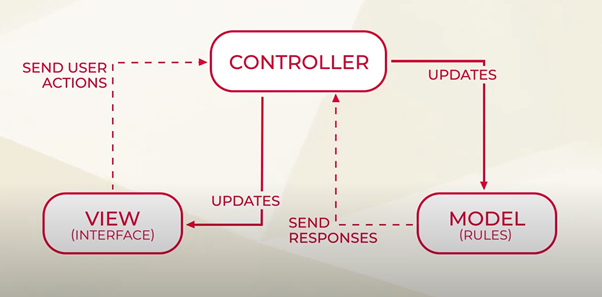
\includegraphics[width=\textwidth]{img/mvc.png} 
\end{figure}

AngularJs has two-way databinding to ease this process. With two-way databinding the model and the view are synchronized. Changes in the model are displayed on the view and vice versa. This means that developers do not have to write code for this purpose, the framework takes care of it. Therefore, the Angular team also defines it's architecture as Model-View-Whatever.

\autocite{Rauh}

\begin{figure}[h!]
    \caption{Two-way databinding}
    \centering
    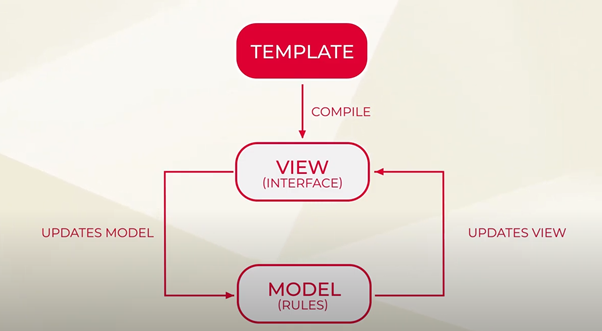
\includegraphics[width=\textwidth]{img/twowaydata.png} 
\end{figure}



\subsubsection{Dependency injection}
Another strength of AngularJs is dependency injection. An application traditionaly exists of different pieces of code that are related to each other.  Instead of attaching dependencies to objects, injectors are used that link these objects to dependencies stored in a central place. This improves the possibility for writing reusable code and isolated unit testing. \autocite{AltexSoft} This way dependency injection allows high cohesion and loose coupling between pieces of code. \autocite{Sterkowitz}


\subsubsection{Directives}
Further AngularJs provided directives as a popular feature. With directives it is possible to add behaviour to a HTML element which allows creating dynamic content. \autocite{AngularJs}

\subsubsection{Downside}
This set of features made AngularJs a good tool for creating SPA's. Though the framework opened a lot of possibilities, it suffered from performance issues when creating large SPA's. One of AngularJs' competitors, React, rolled back to one-way databinding and introduced components to deal with this issue. \autocite{AltexSoft}
\begin{figure}[h!]
    \caption{One-way databinding}
    \centering
    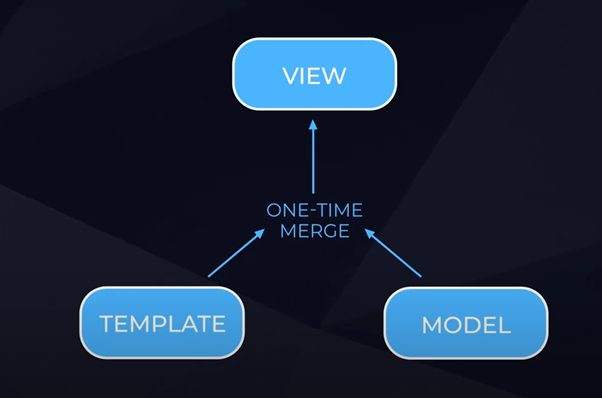
\includegraphics[width=\textwidth]{img/onewaydata.png} 
\end{figure}

\subsection{Angular}
\subsubsection{The update}
The rising popularity of React required the AngularJs team to improve. In September 2016 Google released Angular 2. For now every version starting from Angular 2 is referred to as Angular. AngularJs is every version beneath Angular 2. The reason this naming is important is because of the breaking changes Angular 2 introduced. It is not possible to automatically update AngularJs to Angular and the migrations require a lot of rework.
\autocite{Semenas2020}

\subsubsection{Improved databinding}
In response to the one-way databinding React used, Angular lets the developer define the communication between the component and it's template. The supported types of databinding are:
\begin{itemize}
    \item One-way
    \item Two-way
    \item Event
    \item Property
\end{itemize}
\autocite{AltexSoft}
\subsubsection{Modules and components}
One of the key principles of Angular is the division of an application in modules and components.
Angular is component based like React. The introduction of hierarchical components was a welcome change to deal with the performance issues and it improved code reusability as well. A component traditionally lives in a module, though with newer versions it is also possible to create stand-alone components which is still an experimental feature.
Every Angular application has a root module which takes care of the application startup. An application typically contains a set of feature modules and a shared module. Angular modules can import functionality from and export functionality to other modules. With a shared module it is possible to let feature modules not depend on each other. Organizing the application into distinct modules helps in designing for reusability. The division in modules also takes advantage of lazy-loading, this means only loading a module when it is needed, so the amount of code that needs to be loaded at startup is minimized. 
\autocite{Angular.io}

\begin{figure}[h!]
    \caption{Angular component structure}
    \centering
    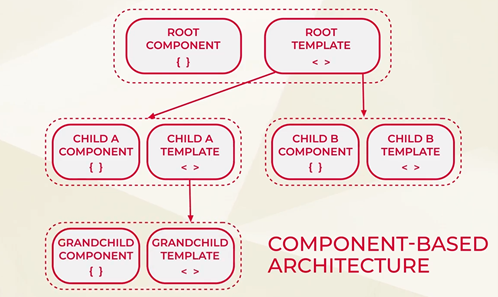
\includegraphics[width=\textwidth]{img/angularcomponent.png} 
\end{figure}

\subsubsection{State management}
Additionally Angular contains a useful library called NgRx that functions as a state and data management tool. NgRx stands for 'Angular reactive extensions' and provides a state management solution based on redux for the Angular ecosystem. In Angular each component has one state and no idea of other component's states. NgRx allows to share this state by keeping it in a single store. This principle is also called the single source of truth. When no state management is implemented, the data is fetched from the back-end server each time a user navigates to the component where the data is shown. When the user modifies the data by performing a CRUD (Create, Read, Update, Delete) operation, the front-end makes a HTTP call to the server to save the modified data and then makes another call to recieve the latest state of the data. The data is stored in the component and lives along with the lifecycle of the component. When the component is destroyed by navigating to another component, it's data is cleared and should be fetched again from the server the next time the component is initialized. NgRx allows to reduce the number of unnecessary requests to the server by creating an in-memory database which contains data that is independent of the lifecycle of any component. This way the data that is fetched, survives during navigations in the application. This may improve the user experience because less loading indicators have to be displayed when data is already loaded. Instead, the modifications a user made are immediately reflected on the screen and saved to the server in the background. As developers don't want to write specific logic for all edge cases, NgRx contains a set of tools that can speed up development. There are five key concepts NgRx is based upon:
\begin{enumerate}
	\item Store
	\item Actions
	\item Reducers
	\item Selectors
	\item Effects
\end{enumerate}

A \emph{store} is a controlled state container mainly for managing global state across an entire application. It contains an observable of state and an observer of actions. \emph{Actions} describe unique events that are dispatched from components and services. Eg: When a user creates a new instance of an entity, a create action is called to add the object to the store. \emph{Reducers} are pure functions that take the current state and latest action as input and provide a new state as output. \emph{Selectors} are pure functions used to select slices of store state. Because the selectors are pure functions, the last result can be returned when arguments match so the functions doesn't have the need to be reinvoked. This practice is known as memoization and can provide performance benefits. \emph{effects} provide a way to interact with services and isolate those services from the components. In the effects, tasks such as fetching data and other external interations are handled. Effects perform tasks and return a new action. This way side effects are isolated from components, allowing for more pure components.

\autocite{AltexSoft}
\begin{figure}[h!]
    \caption{NgRx mechanism}
    \centering
    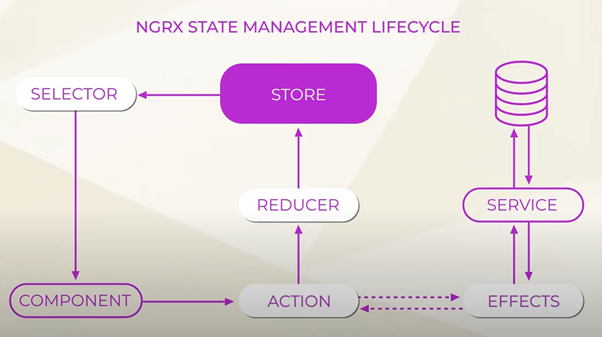
\includegraphics[width=\textwidth]{img/ngrx.png} 
\end{figure}

\subsubsection{Automatic change detection}
Moreover Angular uses Zone.Js to provide automatic change detection. When a model's state has changed, the Angular change detection updates the view to ensure the user interface is synchronized with the latest state of the model.
\autocite{Kumar2020}

\subsubsection{Typescript}
Another important change was that Angular now used Typescript instead of Javascript. Typescript provides static typing which makes it easier for developers to find mistakes before production and use Intellisense to speed up the development process. Typescript is also easy to read for developers with knowledge of Javascript and supports Javascript libraries. In fact, it assembles back to Javascript when compiling.
\autocite{Typescriptlang}

\subsubsection{Hierarchical dependency injection}
One more advantage over AngularJs is that dependency injection became hierarchical. A hierarchical dependency injection system allows to define different scopes for dependencies to run in and follows the component tree structure. This allows to create services that are not application wide but isolated to a subset of components.
\autocite{Rylan}
\begin{figure}[h!]
    \caption{Hierarchical dependency injection}
    \centering
    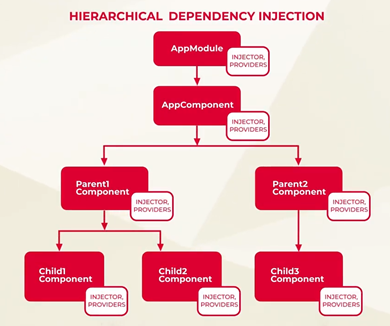
\includegraphics[width=\textwidth]{img/hieradi.png} 
\end{figure}

\subsubsection{Downside}
Many beginners will define Angular as a complex framework to start with. The framework contains lots of features and possibilities. This causes a steep learning curve. The Angular team provides continuous support and new features regularly which is welcomed by experienced developers on the one hand but makes the learning process more difficult for beginners on the other hand.
\autocite{AltexSoft}

\section{Change detection strategies in Angular}
\subsection{Default}
By default, Angular uses Zone.js to trigger change detection. Zone.js does not detect changes itself, instead the responsibility of Zone.js is notifying Angular when to run change detection. \autocite{Inatomi2020} The Angular change detection mechanism then loops over the component tree (starting from the top) to check for changes.
\begin{figure}[h!]
    \caption{Default change detection mechanism}
    \centering
    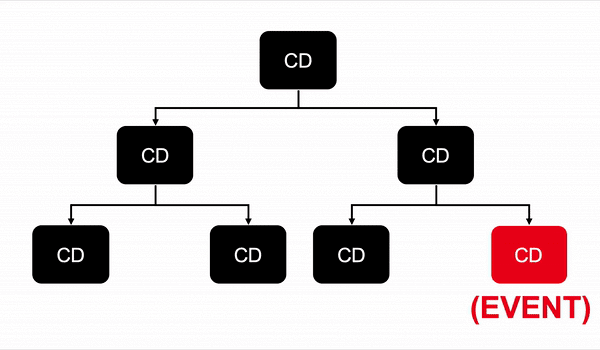
\includegraphics[width=.49\textwidth]{img/cycle1.png} 
    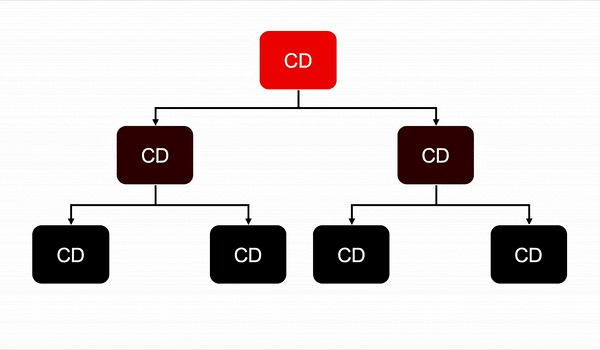
\includegraphics[width=.49\textwidth]{img/cycle2.png} 
    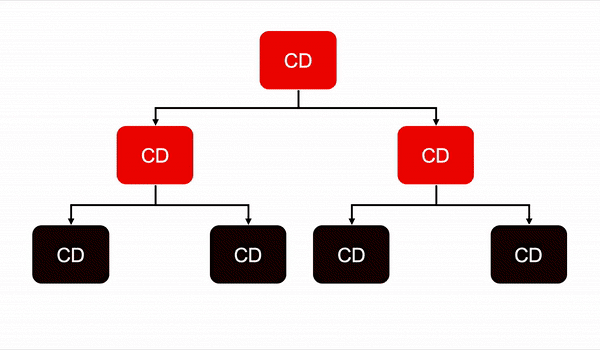
\includegraphics[width=.49\textwidth]{img/cycle3.png} 
    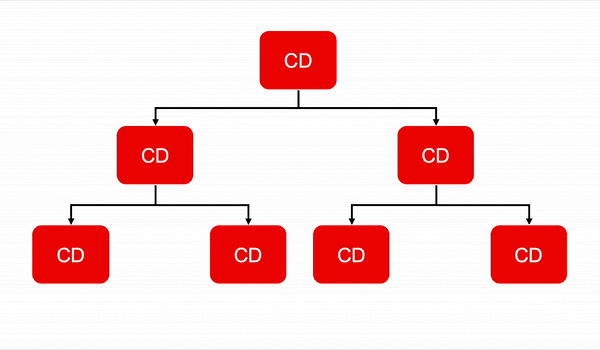
\includegraphics[width=.49\textwidth]{img/cycle4.png} 
\end{figure}

\subsection{OnPush}
With the \emph{OnPush} strategy it is possible to skip components when checking the component tree for changes. When \emph{OnPush} is used, the mechanism follows these steps:
\begin{enumerate}
    \item An event triggers the change detection.
    \item Change detection checks the component tree top to bottom, but skips the parts where \emph{OnPush} is used.
    \autocite{Hoffmann2019}
\end{enumerate}

\begin{figure}[h!]
    \caption{OnPush change detection mechanism}
    \centering
    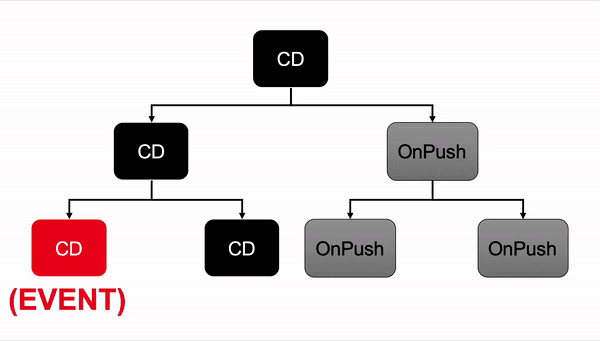
\includegraphics[width=.49\textwidth]{img/onpush-cycle1.png} 
    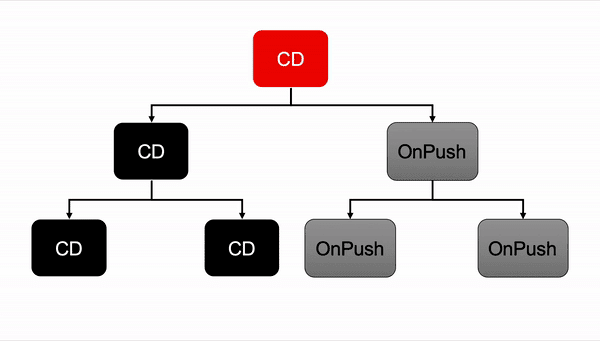
\includegraphics[width=.49\textwidth]{img/onpush-cycle2.png} 
    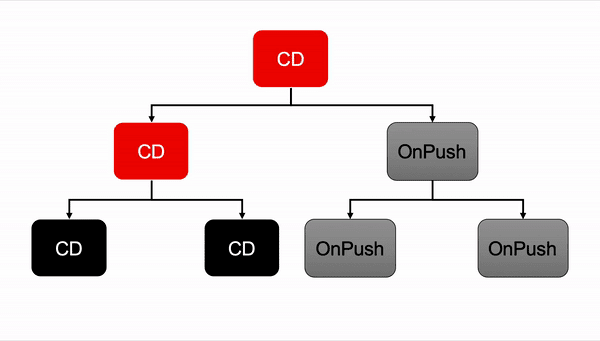
\includegraphics[width=.49\textwidth]{img/onpush-cycle3.png} 
    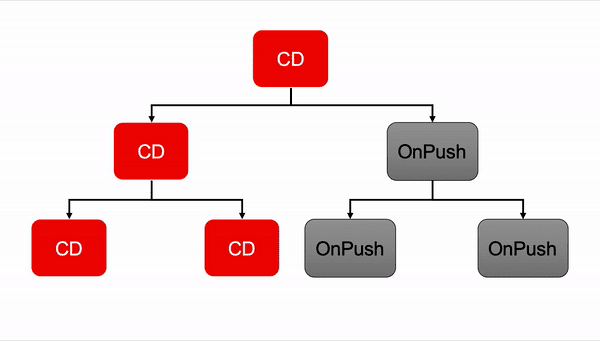
\includegraphics[width=.49\textwidth]{img/onpush-cycle4.png} 
\end{figure}

Thanks to the custom strategy implemented by the developer, Angular will not update the components where \emph{OnPush} is defined unless:
\begin{itemize}
    \item The reference of an \emph{@Input} property changes.
    \item An event handler is triggered in the component or one of its children.
    \item An observable that uses the \emph{async} pipe in the template provides a new value.
    \item The change detection is triggered by the developer.
\end{itemize}
\subsection{Zoneless}

\section{Angular Ivy}
\subsection{Definition}
According to \textcite{Angular.io-ivy} is Ivy the code name for Angular's next-generation compilation and rendering pipeline. With the version 9 release of Angular, the new compiler and runtime instructions are used by default instead of the older compiler and runtime, known as View Engine.

\subsection{Compiler}
The Angular framework is a compiler. A component is written in Typescript and it's template is written in HTML with some additional Angular syntax (directives). When building, Angular compiles this code to a set of Javascript instructions who are able to create and modify the DOM when a component is rendered on the page. If Angular was a car, the compiler would be the engine.

\subsection{Most important features}
The release of Ivy opens up a lot of new potential features. Most of these features are still experimental as the Angular does not want to introduce breaking changes with the new update. Experimental methods are marked with the Greek letter \(\Theta\) (Theta) so developers know this could cause issues when updating. The most important features of Angular Ivy are:
\begin{itemize}
    \item Better build times by ahead-of-time (AOT) compilation
    \item Smaller bundle size by improved tree-shaking
    \item Metaprogramming by using higher order components \autocite{Savkin2018}
    \item Lazy loading of components by using stand-alone components
    \item New change detection system without Zone.js
    \item Ease the publishing process of libraries to NPM
\end{itemize}

\autocite{Exbrayat2019}


\section{Zone.js}
A zone is an execution context that persists across async tasks. Zone.js provides an execution context, lifecycle hooks and a generic error handler for async operations. An execution context is an abstract concept that holds information about the environment where the current code is executed. When a function is excecuted in the JavaScript engine, there will be a new execution context which will determine the scope of variables and functions that can be accessed. Further it will determine the value of the keyword ‘this’. In the JavaScript engine, the value of 'this' depends on the function or class where it is called.

One of the key concepts of zone.js is to provide an additional execution context, another ‘this’, further referred to as 'zoneThis'. The zone context does not replace the basic JavaScript context, but adds a simplified way to handle asynchronous code. When running inside the JavaScript engine, the context changes depending on how and where the function is executed. In zone.js the ‘zoneThis’ will preserve the execution context across asynchronous operations. The ‘zoneThis’ thus will not change as long as it is running within the same zone. For a synchronous operation, ‘zoneThis’ will be the zone it is running in. For an asynchronous operation, ‘zoneThis’ will be the zone where the operation is scheduled. ‘ZoneThis’ does noy really exists, the correct syntax to get the current execution context in Zone.js is Zone.current.
Zone.js also provides interceptable lifecycle hooks:
\begin{itemize}
	\item onFork
	\item onIntercept
	\item onInvoke
	\item onHandleError
	\item onScheduleTask
	\item onInvokeTask
	\item onCancelTask
	\item onHasTask
\end{itemize}

In the following code example the usage of onInvokeTask is demonstrated:
\begin{lstlisting}[language=Javascript]
	ZoneA = {
		onInvokeTask: (callback) => {
			performance.start();
			callback();
			performance.end();
		}	
	};
	ZoneA.run(() => {
		performance.start();
		a();
		setTimeout(c);
		setTimeout(d);
		b();
		performance.end();
	});
\end{lstlisting}

\section{Typescript Decorators}

\section{SignalR}
